\section{Theoretical background}
\begin{frame}{Theoretical background}
\begin{columns}
\begin{column}{0.5\textwidth}
% In this section theory and models of gene regulation are discussed, with models used for different types of inference goals and varying assumptions. Relevant previous work leading to the analysis are covered.
Signal transduction
\begin{itemize}
    \item Phosphorylation
% Signal transduction inside the cell is mostly performed through the addition or removal of phosphates as phosphorylation or dephosphorylation of proteins, although there are many other types of signal transduction and protein regulation such as G-protein coupled receptors mediating trans-membrane signals, second messengers such as calcium ions and lipid messengers. 
    \item TF, $\text{KP} = \text{PK} \cup \text{PP}$, V (any genes)
% For intracellular signals leading to gene regulation, gene regulatory proteins can broadly be categorizes as either transcription factors, kinases or phosphatases, where the TFs have direct effects on the gene transcription and kinases and phosphatases regulates the activity of TFs as well as each other. TFs and their regulons, which are the set of genes regulated by a TF, are largely known, while kinase regulation is not as well documented.

% There are about a factor of 10 less phosphatases of yeast than kinases. They have a much smaller specificity in regulation targets and can, to some extent, be seen as serving a general clean-up role by removing phosphates from regulated proteins in order to let cellular signals decay.
% Phosphorylation can generally be seen as a on/off switch for a specific site on the protein, with one state of phosphorylation inducing an active conformation while the other stabilizes a more inactive conformation. It is atypical that a transcription factor will regulate one set of genes while phosphorylated and another while dephosphorylated. It can both be a phosphorylation that activates a proteins function or deactivates it, however since kinases have more specificity, kinase chains will often send a cellular signal when phosphorylated and have the signal decay with dephosphorylation mediated by phosphatases. Proteins are often modeled as either being on or off, but multiple post-translational modifications can have combined effects leading to multiple levels of protein activity for a given protein.
\end{itemize}

Mutant RNA measurements
\begin{itemize}
    \item Gene deletions reveal indirect insight
% indirect insight
    % Gene deletion, or knockouts, can reveal insight into gene regulation even through RNA expression measurements are not a direct assay for protein-DNA or protein-protein interactions.
% figure
    % If the gene expression levels are observed relative to wildtype we can observe how a gene's expression is affected by the presence or absence of a regulator~(\autoref{fig:gene_deletion}). The direct regulation effects of transcription factors are more straightforward than the indirect effects of a protein kinase. Both edges cannot be inferred from any single knockout experiment even for this simple regulation example. By combining the observation in both an experiment with PK deleted and another with the TF deleted the signs of both edges can be determined, where +1 symbolizes activation and -1 repression. In this manner we can infer edges based on gene expression levels observed to be significantly up- or downregulated compared to wildtype in each of these four patters. The example here is simplified to not include any other regulators which can complicate the edge inference, e.g. if there is another regulation pathway that works as a backup for transcription of the regulated gene, so a robust inference method cannot be basing inference on individual regulation paths in isolation.
    
    \item Vital genes
% A protein chosen to be knocked out might be vital to the functioning of the cell, making it impossible to have any mutant cells to observe. When this is the case a researcher can apply a conditional knockout where the gene can be down-regulated in a time-dependent manner so the measurements can be gathered at a specific time after inducing the knockout and before the death of all cells.

% genes where the mutant is not visibly different than wildtype due to low expression of the gene under the tested conditions
% \textbf{Low wildtype expression at tested conditions}

% There can be issues with genes expressed at low levels in the wildtype under the experimental conditions. If the expression is already low for the wildtype it can be difficult to tell the level apart in a knockout mutant given the noise of microarray measurements. For this reason it has been argued~\cite{ChuaPNAS2006} that overexpression of transcription factors is better than knockouts for transcription factors that might not be expressed at the tested environmental conditions. According to their tests overexpression is good enough to produce noticeable changes even for some transcription factors that would normally not be active under the tested environmental conditions.
% A counterpoint can be made with Savageau’s rule of demand~(\autoref{sec:demand_rule}).

    \item Savageau's rule of demand~\cite{Shinar2006}
\label{sec:demand_rule}
% We consider Savageau’s rule of demand which states that high demand genes are generally induced, and low demand genes repressed under typical conditions. Another way of phrasing it is that genes are bound by their regulators at most times. The rule is established empirically as well as from the evolutionary intuition that it creates the highest selection pressure against unfavorable mutations~\cite{Shinar2006}. If it was the opposite case, where genes were generally not bound by their regulators under typical conditions, a mutation of a regulator could have a less noticeable effect. 
\begin{itemize}
    \item KOs are noticeable
% If Savageau's rule of demand holds, a transcription factor will most likely not be expressed at a near undetectable level under typical conditions, so we would expect a knockout of said TF to have a noticeable effect. In the case of overexpression experiments the expression levels will be noticeably different from wildtype if the transcription is not already saturating the target gene promotor. That will typically not be the case for activating TFs where there would be a 2 to 4 fold increase in expression, but in the case of repressors the promotor can be close to saturated and the effect of TF overexpression can be harder to detect.

% If Savageau's rule of demand does \textit{not} hold, so the promotor of a gene is more often bound by a TF under atypical conditions, it will be harder to detect deviation from wildtype expression levels when the TF is under- or overexpressed. TFs responding to stress and alternative carbon sources and their regulons appear to often violate Savageau’s demand rule so their regulation could be missed if not studied under the appropriate conditions.
\end{itemize}
\end{itemize}



\end{column}
\begin{column}{0.5\textwidth}
\begin{figure}[ht]
    \centering
    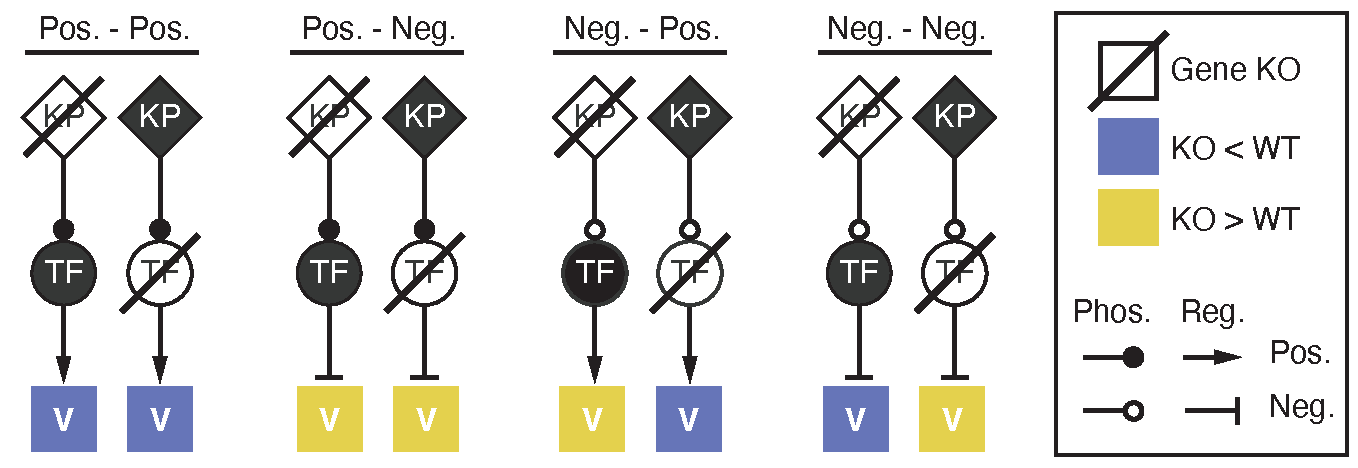
\includegraphics[width=\textwidth]{theory/fig/Fig1.pdf}
    \caption{\textbf{Effect of gene deletion on gene expression.} Gene expression levels relative to wildtype when a KP or TF is knocked out.}
    \label{fig:gene_deletion}
\end{figure}
\end{column}
\end{columns}
\end{frame}


\begin{frame}{Modelling cooperativity}
\begin{columns}
\begin{column}{0.4\textwidth}
% For the simple case of a single transcription factor regulating the transcription rate of a single gene, the number of protein molecules produced of the regulated gene per unit time is a function of the concentration of the transcription factor in its active form~\cite{Alon2006}.
% The Hill equations~(\autoref{eq:Hill}) describe the cooperativity of binding for ligands to a receptor or for a similar binding event, for instance the binding of TFs to a regulatory region of DNA. The Hill equation is given here for the case of a single activator~(\autoref{eq:Hill_activator}) and a single repressor~(\autoref{eq:Hill_repressor}).
Single transcription factor regulating a single gene~\cite{Alon2006}
\begin{subequations}
\label{eq:Hill}
\begin{align}
\label{eq:Hill_activator}
\theta_{\text{activator}} &= \frac{p_j^{\nu_j}}{k_j^{\nu_j} + p_j^{\nu_j}} = \frac{\chi_j}{1 + \chi_j}
\\
\label{eq:Hill_repressor}
\theta_{\text{repressor}} &= \frac{1}{1 + \left(\frac{p_j}{k_j} \right)^{\nu_j}} = \frac{1}{1 + \chi_j}
\\
\chi_j &=
\left( \frac{p_j}{k_j} \right) ^ {\nu_j}
\end{align}
\end{subequations}
% Here $p_j$ is the ligand concentration (concentration of the $j$-th protein), $k_j$ and $\nu_j$ are model parameters. Different values for $k_j$ and the Hill coefficient $\nu_j$ determines $\theta$, which is the fraction of maximum transcription if regulated by either a single activator or repressor. If the concentration of ligand is $p_j = k_j$ then there will be half occupancy of the receptor. The basic assumption is that we use the fraction of occupancy of bound receptor~(the promotor of a gene), to describe transcription rate. The equations are sometimes multiplied by a constant $r_\text{max}$, which holds the maximum transcription rate unique to a given gene. This way $\theta$ will be the absolute instead of relative transcription rate, and have the dimension of $r_\text{max}$ instead of being dimensionless.


\end{column}
\begin{column}{0.6\textwidth}
\begin{figure}[ht]
\centering
\begin{subfigure}[b]{0.49\textwidth}\centering\caption{}
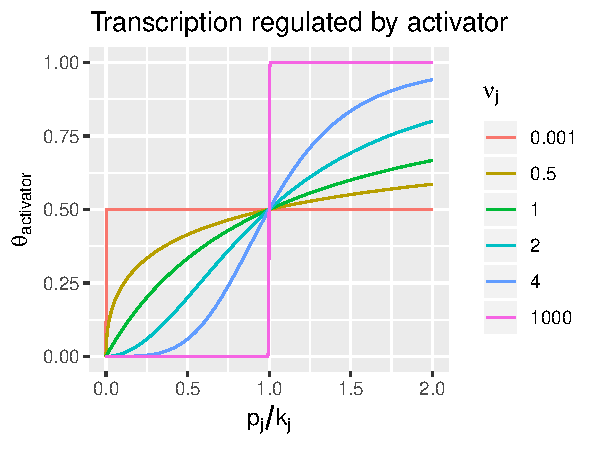
\includegraphics[width=\textwidth]{theory/fig/hill_activator.pdf}
\end{subfigure}
% \vskip\baselineskip
\begin{subfigure}[b]{0.49\textwidth}\centering\caption{}
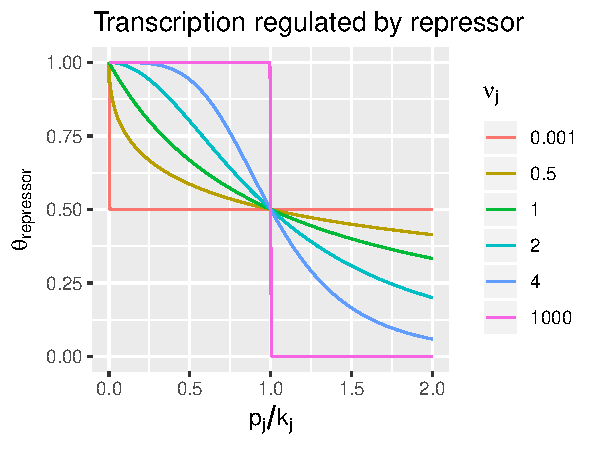
\includegraphics[width=\textwidth]{theory/fig/hill_repressor.pdf}
\end{subfigure}
\caption{\textbf{Hill equation models of gene regulation.} Single activator~(a), and repressor~(b).
% Unique curves result from using different model parameters $\nu_j$. 
}
\label{fig:Hill}
\end{figure}
% The equations are designed to capture cooperation in ligand binding as well as a receptor becoming saturated with increased ligand concentration~(\autoref{fig:Hill}).
% $\nu_j=1$ means that the receptor gets saturated linearly, $\nu_j<1$ means negative cooperation where it is more resistant to binding of ligand if some is already bound, and $\nu_j>1$ is positive cooperation. 
\end{column}
\end{columns}
\end{frame}


\subsection{Modelling gene expression with differential equations}
\begin{frame}{Modelling gene expression with differential equations}
% Transcription and translation kinetics are often modelled using differential equations~\cite{Chen99}. We can model the dynamic as~\autoref{eq:Chen99}, if we assume the process of transcription and translation takes a negligible amount of time, so the effect of regulation becomes instantly apparent in the rates of molecule production.
Chen et al.~\cite{Chen99}
\begin{subequations}
\label{eq:Chen99}
\begin{align}
\dv{\boldsymbol{r}}{t} &=
f(\boldsymbol{p}) - \Lambda_\text{RNA} \boldsymbol{r}
\\
\dv{\boldsymbol{p}}{t} &=
M \boldsymbol{r} - \Lambda_\text{Prot} \boldsymbol{p}
\end{align}
\end{subequations}
% Here, $\boldsymbol{r}$ is a vector of mRNA concentrations $r_i$ for each gene $i$, $\boldsymbol{p}$ is similarly a vector of protein concentrations for each gene $i$. $\Lambda_\text{RNA}$ and $\Lambda_\text{Prot}$ are diagonal matrices holding decay rates for each mRNA or protein, $M$ is a matrix with values for linear rates of protein production from the relevant coding mRNA, and $f$ is some function for how mRNA rates are influenced by each of the protein concentrations. Chen~et~al. argues for the application of using $f(\boldsymbol{p}) = C \boldsymbol{p}$ with a Taylor approximation and defines the solution to the ordinary linear system of differential equations. 

% Differential models describing time-dependent kinetics of transcription and translation regulation can be readily applied to time series data. It can be done by assuming that the intervals between measurements are short enough that the differential can be approximated with the differences between measurements at each time step, however real-time measurements are collected at a lower rate than the time scale of biological interaction.

% Differential equations has been used for modelling gene regulation with multiple transcription factors with both linear and nonlinear gene regulation, for instance by Anderson~et~al.~\cite{Anderson2009}, who modeled transcription factor concentrations as Gaussian Processes which are stochastic processes, purely defined by a mean and covariance term~(\autoref{eq:gaussian_process}).
Gaussian Processes~\cite{Anderson2009}
\begin{subequations}
\label{eq:gaussian_process}
\begin{align}
\dv{\boldsymbol{r}}{t} &=
\boldsymbol{r}_0 + C \boldsymbol{p} - \Lambda_\text{RNA} \boldsymbol{r}
\\
p_i &= f_i(t) =
\mathcal{GP}\left(0, \exp(-\frac{(t-t')^2}{l_i^2})\right)
\end{align}
\end{subequations}
\begin{itemize}
% Here, $\boldsymbol{r}_0$ is a vector with basal transcriptional concentrations for each gene, $p_i$ is the $i$-th element of the protein concentration vector $\boldsymbol{p}$ which describes the concentrations of transcription factors as a Gaussian Process $\mathcal{GP}$ with mean 0 and covariance as an exponential function. $l_i$ is a hyperparameter of the model, which was chosen to be 0.1 for one example of simulation. Modelling the transcription factors as a Gaussian Process leaves out regulatory effects onto transcription factors, so the model was further extended to describe a cascade of transcription factors, each regulating the gene of the next transcription factor in the cascade. The models were not extended to protein kinases. 
    \item \textcolor{darkgray!50!gray}{models for time series gene expression $\rightarrow$ GP parameters}
% The models are in this case used for inferring the parameters defining the underlying Gaussian Processes for the transcription factor concentrations, that were giving rise to the observed gene transcription levels. It assumes adequate amounts of time series data for the gene transcripts, and does not directly infer which transcription factors regulate which genes, but rather assumes it is known.
    \item \textcolor{darkgray!50!gray}{intentions of generalization, using TF concentration $\rightarrow$ TF interactions}
% If the model could be generalized to describing any combination of transcription factors and designed to utilize TF concentrations, it might be possible to infer which transcription factor interactions are present. 
\end{itemize}
\end{frame}

% \subsubsection{GeneNetWeaver}
\begin{frame}<1>[label=gnw]
\label{sec:dream}
\begin{columns}
\begin{column}{0.53\textwidth}
\alt<1>{
\frametitle{GeneNetWeaver}
\begin{itemize}
    \item Simulating gene expression in Java
    \item Used in DREAM challenge for benchmarking inference
    \item Regulation model:
\end{itemize}
% Modelling gene expression with differential equations has been applied to benchmark different attempts at inferring which transcription factors regulate which genes. The DREAM~(Dialogue for Reverse Engineering Assessments and Methods) challenges are organised by a variety of researchers from multiple organizations putting forward a challenge open to the public and assessing attempts at a solution. "DREAM4" was a challenge in reverse-engineering an in silico gene regulation network from gene expression levels. Gene expression levels were simulated, instead of collected experimentally, in order for the true underlying interactions to be definitively known.
% The simulation was intended to be biologically realistic and was simulated using the Java software GeneNetWeaver applying a nondimensionalized model defined as the differential equations in~\autoref{eq:gnw_main}, which are clearly similar to the differential equations in~\autoref{eq:Chen99}.
\begin{subequations}
\label{eq:gnw_main}
\begin{align}
\label{eq:gnw_main.a}
\dv{r_i}{t} &=  m_i^{(\text{RNA})} f_i(\boldsymbol{p}) - \lambda_i^{(\text{RNA})} r_i \\
\dv{p_i}{t} &=  m_i^{(\text{Prot})} r_i -  \lambda_i^{(\text{Prot})} p_i
\end{align}
\end{subequations}
% The values $m_i^{(\text{RNA})}$ and $m_i^{(\text{Prot})}$ are the maximum transcription and translation levels for the $i$-th protein. The function $f_i$ describes the expected fraction of maximum transcription for gene $i$ given nondimensionalized protein concentrations $\boldsymbol{p}$, so it holds $f_i(\boldsymbol{p}) \in [0,1]$.
% $f_i$ is mentioned in supplementary material of~\cite{Marbach2010} and based on the work in~\cite{GeneNetWeaverModel}. It takes into account different types of gene regulation, both regulator interactions and cooperation for any combination of activators and repressors~(\autoref{fig:gnw_regulation}).
% A gene has a set of binding sites, each affecting its transcription level. Each of the TFs regulating gene $i$ can bind to only one binding site in the GeneNetWeaver model. The TF can bind to the binding site with dynamics built on Hill equations~(\autoref{eq:Hill}). The effect of a bound site on gene transcription rate can be flipped in the model, indicated for site $m=2$ in~\autoref{fig:gnw_regulation}, where TFs binding the site using dynamics inspired by activator Hill equations~(\autoref{eq:Hill_activator}) has a repressing effect on the transcription rate of gene $i$.
}{
\stepcounter{equation}
}
\only<2>{
\frametitle{GeneNetWeaver - Example}
% The terms defined in~\autoref{eq:gnw_f} are calculated using the example shown in~\autoref{fig:gnw_regulation} for illustrative purposes:
\begin{subequations}
\begin{align*}
N &= 3
\,,\,
C = \{3\}
\\
A_1 &= \{1\}
\,,\,
A_2 = \{4\}
\,,\,
A_3 = \{5,6\}
\\
R_1 &= \emptyset
\,,\,
R_2 = \{2,3\}
\,,\,
R_3 = \emptyset
\\
\mu_1 &= \frac{\chi_1}{1 + \chi_1}
\\
\mu_2 &= \frac{\chi_4}{1 + \chi_4 + \chi_2 \chi_3 \chi_4}
\\
\mu_3 &= \frac{\chi_5}{1 + \chi_5} \frac{\chi_6}{1 + \chi_6}
\\
\sigma_1 &= \emptyset
\,,\,
\sigma_2 = \{1\}
\,,\,
\sigma_3 = \{2\}
\,,\,
\sigma_4 = \{1,2\}
\\
\sigma_5 &= \{3\}
\,,\,
\sigma_6 = \{1,3\}
\,,\,
\sigma_7 = \{2,3\}
\,,\,
\sigma_8 = \{1,2,3\}
\\
P\{\sigma_1 | \boldsymbol{p}\} &= (1 - \mu_1) (1 - \mu_2) (1 - \mu_3)
\\
P\{\sigma_2 | \boldsymbol{p}\} &= \mu_1 (1 - \mu_2) (1 - \mu_3)
\\
P\{\sigma_3 | \boldsymbol{p}\} &= (1 - \mu_1) \mu_2 (1 - \mu_3)
\\
...
\\
P\{\sigma_8 | \boldsymbol{p}\} &= \mu_1 \mu_2 \mu_3
\end{align*}
\end{subequations}

}
\end{column}
\begin{column}{0.47\textwidth}

\begin{figure}[ht]
  \centering
  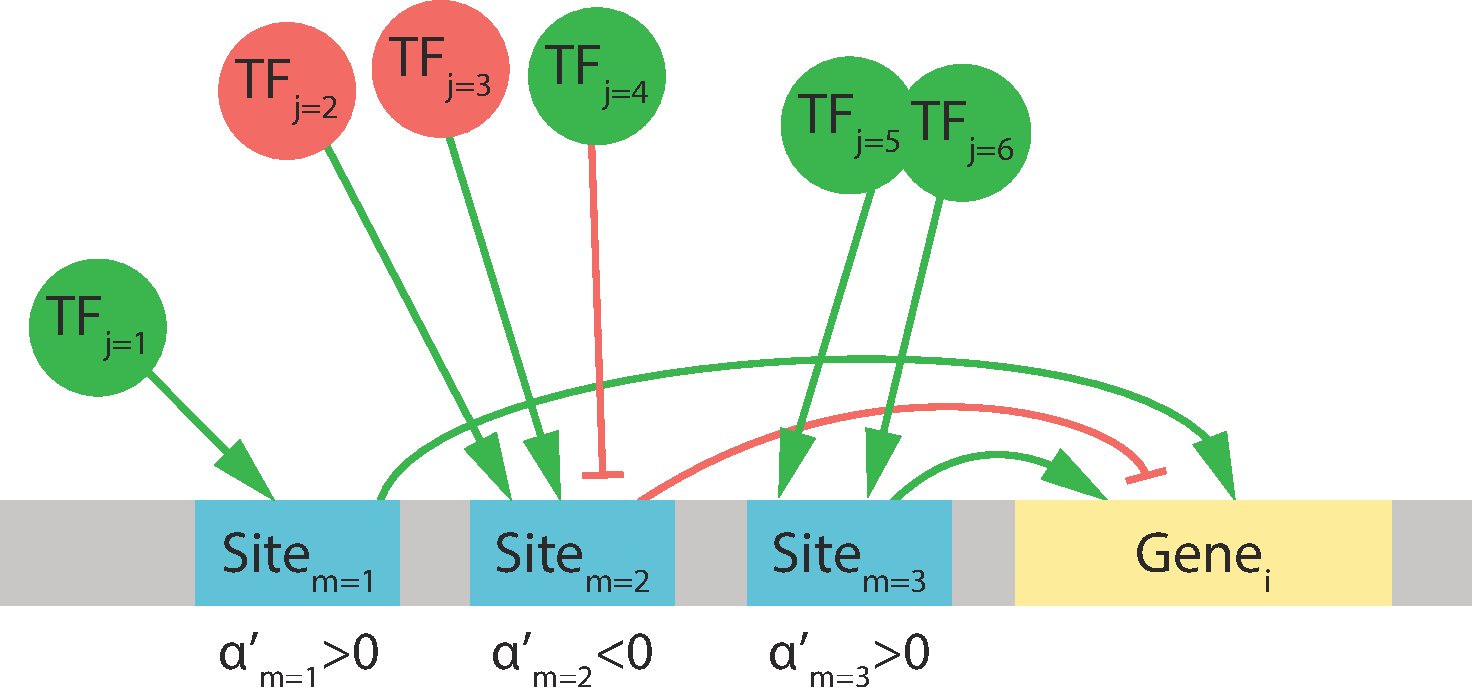
\includegraphics[width=\textwidth]{theory/fig/GeneWeaverRegulation.pdf}
   \caption{\textbf{Example of transcriptional regulation in simulation.}
    A gene regulated by $N=3$ regulatory modules, where module 1 is regulated by a single activator TF, module 2 is bound by a complex of two TFs, which both have to be present for activation of the module, and activating and repressing TFs compete to bind the third module. \textcolor{OliveGreen}{Green}: activation, \textcolor{red}{red}: repression.} 
  \label{fig:gnw_regulation}
\end{figure}



\end{column}
\end{columns}
\end{frame}

\begin{frame}{GeneNetWeaver - Defining gene regulation}
\begin{columns}
\begin{column}{0.5\textwidth}
% The exact equation for $f$ is unpublished but defined in the source code, and written here in~\autoref{eq:gnw_f}, focusing on the function $f_i$ for a single gene $i$. Each binding site can either be bound by transcription factor(s) or unbound. For $N$ binding sites this creates $2^N$ unique combinations~(\autoref{eq:gnw_f.a}), which we refer to as "states". Each state~$\sigma_s$ for $s \in \{1,2,3,...,2^N\}$ are each defined as a unique combination of bound and unbound binding sites.
\small
Based on Marbach~et~al.~\cite{Marbach2010}, Dassow~et~al.~\cite{GeneNetWeaverModel}
\normalsize
\begin{subequations}
\label{eq:gnw_f}
\begin{align}
\label{eq:gnw_f.a}
f_i(\boldsymbol{p}) &=
\sum_{s=1}^{2^N} \alpha_s P\{\sigma_s | \boldsymbol{p} \}
\\
\label{eq:gnw_f.b}
\alpha_s &=
\alpha_0' + \sum_{m \in \sigma_s} \alpha_m'
\\
\label{eq:gnw_f.c}
P\{\sigma_s | \boldsymbol{p} \} &=
\prod_{m \in \sigma_s} P\{\beta_m=1|\boldsymbol{p}\} \cdot \prod_{m \notin \sigma_s} \left( P\{\beta_m=0|\boldsymbol{p}\} \right)
\\
\label{eq:gnw_f.d}
&=
\prod_{m \in \sigma_s} \mu_m \cdot \prod_{m \notin \sigma_s} \left( 1 - \mu_m \right)
\end{align}
\end{subequations}
$\beta_m$ = module $m$ under activating binding conditions
\end{column}

\begin{column}{0.5\textwidth}
\begin{subequations}
\begin{align}
\label{eq:gnw_f.e}
\mu_m &=
\begin{cases}
  \frac{\prod_{j \in A_m} \chi_j}{\prod_{j \in A_m \vee R_m} 1 + \chi_j},
  & \text{if}\ m \in C \\
  \frac{\prod_{j \in A_m} \chi_j}{1 + \prod_{j \in A_m} \chi_j},
  & \text{if}\ m \notin C \wedge \forall j \in A_m \\
  \frac{\prod_{j \in A_m} \chi_j}{1 + \prod_{j \in A_m} \chi_j + \prod_{j \in A_m \vee R_m} \chi_j},
  & \text{otherwise}
\end{cases}
\\
\label{eq:gnw_f.f}
\chi_j &=
\left( \frac{p_j}{k_j} \right) ^ {\nu_j}
\end{align}
\end{subequations}
% Here, $P\{\sigma_s | \boldsymbol{p}\}$ is the probability that a gene is in regulation state $\sigma_s$ given the current protein concentrations $\boldsymbol{p}$. $\alpha_s$ is the fraction of maximum gene transcription for state~$\sigma_s$, and is computed from the sum of baseline activation and relative activation for each binding site that are bound in the given state $\sigma_s$~(\autoref{eq:gnw_f.b}). It holds $\alpha_s \in [0,1]$.
% If we consider state $\sigma_s$ a set of all binding sites bound when a gene is in said state, then the probability that gene $i$ is in state $\sigma_s$ is defined by the probability of sites in set $\sigma_s$ bound and sites not in $\sigma_s$ unbound~(\autoref{eq:gnw_f.c}). The Boolean $\beta_m$ indicates if site $m$ is bound or not. The probabilities are equivalent to the expected fraction of binding sites bound~(\autoref{eq:gnw_f.d}), which is defined in three different ways in~\autoref{eq:gnw_f.d} depending on whether the binding site is regulated by a TF binding complex~($m \in C$), and if some of the TFs for a binding site are repressors~($\exists j \in R_m$) or if all are activators~($\forall j \in A_m$).
% \autoref{eq:gnw_f.e} is based on Hill equations~(\autoref{eq:Hill}). It can be seen that if a binding site $m$ is only regulated by a single activating TF, then we get $\mu_m = \theta_{\text{activator}}$ from \autoref{eq:Hill_activator} and if only regulated by a single repressing TF, we get $\mu_m = \theta_{\text{repressor}}$ for \autoref{eq:Hill_repressor}. This is the case regardless if $m \in C$ or not, although it does not make sense to describe a lone transcription factor as regulating in a complex.
% \pagebreak
\end{column}
\end{columns}
\end{frame}

\againframe<2>{gnw}

\begin{frame}{GeneNetWeaver - Initial conditions}
% To prepare for the simulation, the GeneNetWeaver software is given an adjacency matrix~(\autoref{sec:graph}) with values indicating which genes each protein regulates. Model parameters are then set randomly, for instance setting random mRNA and protein decay rates. Rate parameters are assigned random values using~\autoref{eq:gnw_param_initial} which describes random decay rates.

\begin{subequations}
\label{eq:gnw_param_initial}
\begin{align}
m_i^{(\text{RNA})} &= \lambda_i^{(\text{RNA})} \sim \frac{\log (2)}{\mathcal{T}(a=5, b=50)} \\
m_i^{(\text{Prot})} &= \lambda_i^{(\text{Prot})} \sim \frac{\log (2)}{\mathcal{T}(a=5, b=50)}
\end{align}
\end{subequations}

$\mathcal{T}(a,b)$ = normal distribution truncated to $[a,b]$. $a$ and $b$ selected from~\cite{GeneNetWeaverModel}


$\mathcal{T}(a,b)$ has $\mu=\frac{a+b}{2}$, $\sigma=\frac{b-a}{6}$



% Here, $\mathcal{T}(a,b)$ is a normal distribution truncated to the interval $[a,b]$ with $\mu=\frac{a+b}{2}$ and $\sigma=\frac{b-a}{6}$. It serves as descriptor of mRNA and protein half-life. Its range parameters are selected based on~\cite{GeneNetWeaverModel}.


% Gene expression and protein levels are initialized at time zero by letting gradients equal zero as described in~\autoref{eq:initial_gnw}.

\begin{subequations}
\label{eq:initial_gnw}
\begin{align}
\dv{r_i}{t} = 0 &\implies r_i = \frac{m_i^{(\text{RNA})}}{\lambda_i^{(\text{RNA})}}  f_i(\boldsymbol{p})  \\
\dv{p_i}{t} = 0 &\implies p_i = \frac{m_i^{(\text{Prot})}}{\lambda_i^{(\text{Prot})}} r_i
\end{align}
\end{subequations}

% Gene expressions $r_i$ for each gene $i$ are initially set without protein regulation, which means $r_i$ is evaluated here using $\boldsymbol{p} = \boldsymbol{0}$. More initialization code is also run in order to set $\alpha_s$ for each state.


\end{frame}

\begin{frame}{Kinase regulation model}
\label{sec:Heinrich}

\begin{columns}
\begin{column}{0.5\textwidth}


% Protein phosphorylation is a ubiquitous means of regulating protein activity controlled by protein kinases and phosphatases. Kinase cascades allows a signal from outside the cell to propagate into the nucleus via phosphorylation events as modelled by Heinrich~et~al.~\cite{Heinrich2002kinase}.

% The signal can be described as a single activated receptor sending a signal that decays with rate~$\lambda^{(\text{Receptor})}$, and where each protein kinase has a single protein kinase input~(\autoref{fig:kinase_cascade}). The change in phosphorylation of a kinase $i$ is modelled as follows:
Kinase cascade, each protein with single input~\cite{Heinrich2002kinase}
\begin{subequations}
\label{eq:kinase_cascade}
\begin{align}
\dv{\phi_i}{t} &=
    \tilde{w}_i \phi_{i-1} \tilde{\phi}_i - \lambda_i^{(\text{Phos})} \phi_i
\\
    &=
    w_i \phi_{i-1} \left(1 - \frac{\phi_i}{p_i}\right) - \lambda_i^{(\text{Phos})} \phi_i
\\
p_i &= \phi_i + \tilde{\phi}_i
\,,\,
w_i = \tilde{w}_i p_i
\end{align}
\end{subequations}

% Here, $\phi_i$ is the amount of phosphorylated protein $i$ and $\tilde{\phi}_i$ is the unphosphorylated amount. $w_i$ is the kinase rate of phosphorylation by phosphorylated protein $i-1$ on unphosphorylated protein $i$, and $\lambda_i^\text{Phos}$ is the decay rate of the phosphate group on protein $i$, which is controlled by the reaction of all the phosphatases in the cell with protein $i$. 
% It is assumed that a phosphorylation event is always an unphosphorylated kinase being phosphorylated by another kinase which itself is phosphorylated.

% The regulation generalizes to include the possibility of multiple inputs of regulation onto each protein kinase, which can be written with vector notations~(\autoref{eq:kinase_general}).

Generalized, any protein can affect any protein
\begin{subequations}
\label{eq:kinase_general}
\begin{align}
\dv{\phi_i}{t} &=
    \left( \sum_j w_{ij} \phi_j \right) \left(1 - \frac{\phi_i}{p_i}\right) - \lambda_i^{(\text{Phos})} \phi_i
\\
\label{eq:matrix_kinase}
\dv{\boldsymbol{\phi}}{t} &= (W \boldsymbol{\phi}) \left(1 - \frac{\boldsymbol{\phi}}{\boldsymbol{p}}\right) - \Lambda_\text{Phos} \boldsymbol{\phi}
\end{align}
\end{subequations}

% Here $w_{ij}$ is the regulation effect from node $j$ to $i$, which is a positive value. The division in~\autoref{eq:matrix_kinase} is an elementwise division.


\end{column}
% \begin{column}{0.5\textwidth}
% \begin{figure}
% \begin{minipage}[c]{0.42\textwidth}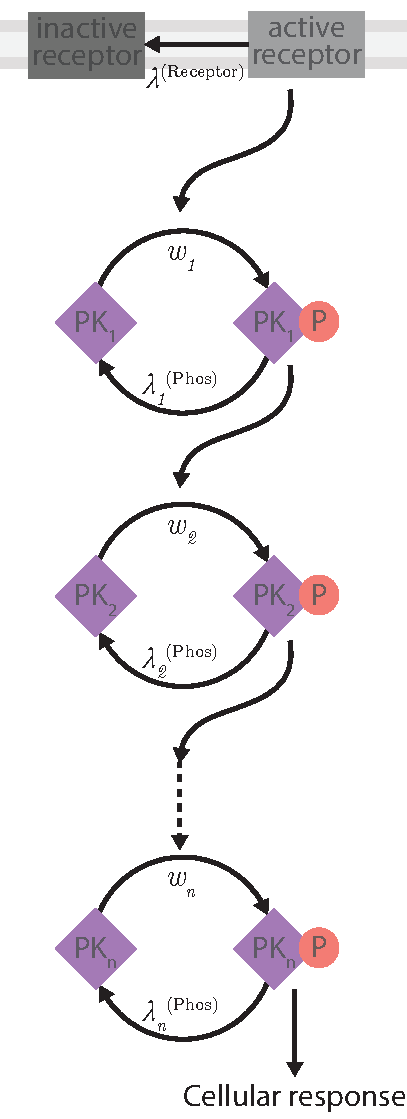
\includegraphics[width=\textwidth]{theory/fig/kinase_cascade.pdf}\end{minipage}
% \begin{minipage}[t]{0.54\textwidth}\caption{\textbf{Kinase cascade with single inputs.} A protein kinase cascade transmitting a signal from a cell membrane receptor.}\end{minipage}
% \label{fig:kinase_cascade}
% \end{figure}
% \end{column}

\begin{column}{0.5\textwidth}
\begin{figure}
\begin{minipage}[t]{0.4\textwidth}
\caption{\textbf{Kinase cascade with single inputs.} Transmitting signal from a membrane receptor.}
\end{minipage}
\begin{minipage}[c]{0.37\textwidth}
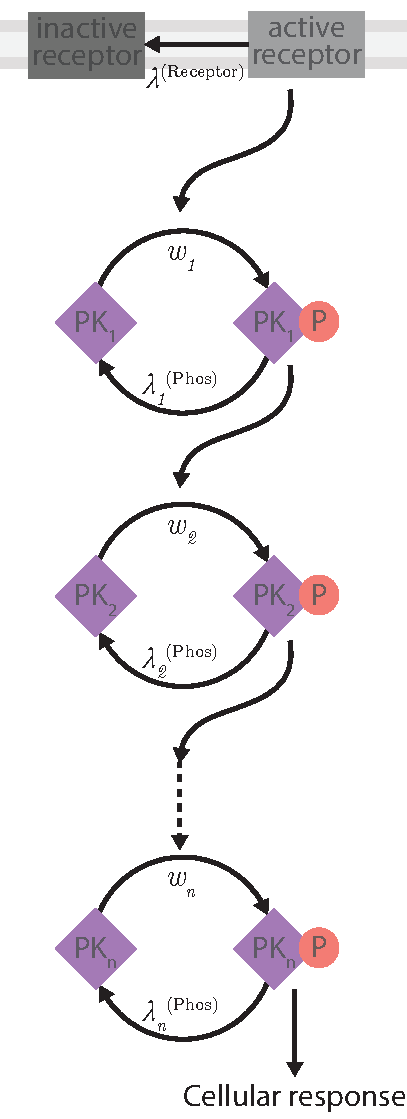
\includegraphics[width=\textwidth]{theory/fig/kinase_cascade.pdf}
\end{minipage}
\label{fig:kinase_cascade}
\end{figure}
\end{column}
\end{columns}
\end{frame}



% \begin{frame}{Graphs}
\label{sec:graph}
Signal transduction network
\begin{itemize}
% graph representation
    \item $\mathcal{G} = \left< \mathcal{V}, \mathcal{E} \right>$
% A signal transduction network in a cell can be represented as a graph $\mathcal{G} = \left< \mathcal{V}, \mathcal{E} \right>$, defined as a set of vertices $\mathcal{V}$ and edges $\mathcal{E}$, where each can be assigned attributes, which often are a single scalar. Typically, an edge connects two vertices (nodes) in a graph and can be either undirected or directed, giving it a source and target node. In a hypergraph an edge can connect more than two nodes, which can be useful for metabolic networks where an edge can represent a reaction, for which there can be multiple input and output metabolites represented as the vertices connected to the edge.
% Edges in a graph representing a protein interaction network can represent the physical binding of proteins or binding of proteins to promotors of genes while nodes represent proteins and genes. Edge attributes can represent regulation strength from TFs to genes, while the node attribute can represent gene product concentration. Genes and their protein products can also be represented as a single node. Separate gene and protein representations are useful if it is not assumed to be known which proteins are coded by which genes. When gene and protein product is a single node ambiguity as to whether an edge is regulating the gene~(transcriptional regulation) or the protein~(protein-protein interaction), can be avoided either with an explicit edge attribute signifying its type of interaction, or by basing the type of interaction on the source node of the edge. The latter can be done if a protein is either strictly classified as a transcription regulator or as a protein regulator. Genes and proteins as separate or combined node representations has both been used in this project. A gene and its protein product were separate in~\autoref{sec:convergence_model}, but otherwise considered a single node.
    \item adjacency matrix
% A Graph can be represented as an adjacency matrix where element $i,j$ is the edge from node $j$ to node $i$. The matrix can be symmetrical, which is used to represent an undirected graph where each element represents the connection between two nodes, without influence from choice in $j$ and $i$. Examples of matrices that can be used as a adjacency matrix representation of an undirected graph are covariance, correlation, and partial correlation matrices.

% If the values are restricted to the Boolean case, for instance ones and zeros, it is used for indication of the presence and absence of an edge. Edges with values -1, 0, and 1 can be used to indicate repression, no effect, and activation, respectively. Real value numbers can encode the strength of activation or repression as well. Positive real value numbers can also be used to indicate weighted edges, for instance representing some concept of attraction forces.
\end{itemize}
DAG
\begin{itemize}
    \item paths can be followed to completion
% Directed Acyclic Graphs (DAGs) are a well studied type of graph, used in fields such as machine learning. When a graph is acyclic and directed there exists no path from a node back to itself, that follows the direction of edges. For this reason it is possible to follow any path to completion. Machine learning networks, such as a feedforward network, will be DAGs with a natural progression layer by layer without infinite loops occurring. This makes it possible to define gradients fully describing how each parameter of a model has influence on the value of network outputs in the last layer of the network.
    \item gene regulation is cyclic
% A biological network modelling transcription and translation relies heavily on feedback loops through the transcription and translation of proteins that regulate other iterations of transcription and translation themselves.
% The cycles complicates many aspects of studying the graph, such as describing conditional independence among the nodes~\cite{Tillman2014}.
\end{itemize}
Network inference
% node inference
% Inferring attributes for the vertices of a biological network can be difficult since attributes such as protein or mRNA concentration generally vary a lot depending on cell cycle and environmental factors. Vertex attributes of interest can be the production level or potential production level of a compound for which we are trying to optimize production.
% edge inference
% Inferring the edges of a biological network is an attempt to understand which protein-protein and protein-DNA interactions are taking place, which should be more static than vertex attributes and is what is usually the focus of biological network inference.
% Wanting to find the edges in the network is to say that we are interested in causal connections. As opposed to typical machine learning training of prediction networks we are not interested in finding a nonlinear function mapping from an input to an output as well as possible with a black-box method, but instead to use biological data to shape the causal edges in a network. Predictive performance can however be a secondary objective.
\begin{itemize}
    \item Likelihood based
% Graph learning has been explored using methods maximizing likelihood. Functions are described for the probability of a set of graph edges given observed attributes of the network, and the optimal graph is selected. There are many benefits to a likelihood based approach to edge inference, where the model will describe the basis for inferences and the confidence in them, compared to for instance a "black box" machine learning approach.
% There are also issues with the complexity of likelihood approaches, where graphs with different edges can have equal likelihood of fitting a given dataset, edges might not indicate causality, the amount of data required for a convergent solution grows exponentially with the number of parameters to infer, and heuristics are usually applied to find suboptimal solutions as discussed by Yeang~\cite{Yeang2004}. Yeang goes on to describe and test a model for graph inference where edges are inferred to be present or absent, and if present, inferred to have positive or negative effects of target nodes. The edge strength is used as a p-value to evaluate certainty of predictions. The model is based on log likelihood ratios for hypothesis testing on graph parameters. Knockout data are applied, and the model constrained by protein-protein interaction data and protein-DNA interactions.
\cite{Yeang2004}
% We will combine similar data here, and also use the absolute sizes of predicted edge weights as a score for our belief in the presence in an edge in the graph.
\end{itemize}
\end{frame}


\subsection{Causality and cyclic graphs}
\begin{frame}{Causality and cyclic graphs}
\label{sec:eberhardt}
\begin{columns}
\begin{column}{0.65\textwidth}
% Causal structure learning, where causal edges are inferred on graphs representing real systems, is often performed on DAGs, as described in a review by Heinze-Deml~et~al.~\cite{CausalLearningReview}. DAGs are too simple to use for biological networks where gene transcription products are taken into account. The only model in the review that is designed for cyclic graphs is BackShift, which is an extension of LLC~(Linear, Latents, Cyclic) described by Eberhardt~et~al.~\cite{EberhardtLLC}. Both methods are designed in pursuit of inferring network edges from node attributes observed under different interventions. The interventions are changes to nodes in the graph, which breaks all ingoing edges. In LLC it is assumed to be known which nodes have been intervened on, which is not assumed with BackShift. For knockout studies we know which nodes (genes) have been knocked out, so LLC is discussed here.
% We first assume a system of node values that are controlled linearly by the values from all parent nodes through discreet time steps~(\autoref{eq:eber_linear}).
Eberhardt et al.~\cite{CausalLearningReview}
\begin{subequations}
\label{eq:eber_linear}
\begin{align}
x_i (t) &=
    \sum_j b_{ij} x_j (t - 1) + e_i
\\
\label{eq:eber_linear.b}
\boldsymbol{x}(t) &=
    B \boldsymbol{x} (t - 1) + \boldsymbol{e}
=
    B \left( B \boldsymbol{x} (t - 2) + \boldsymbol{e} \right) + \boldsymbol{e} = ...
\\
&=
    B^t \boldsymbol{x}(0) + \sum_{i=0}^{t-1} B^i \boldsymbol{e}
\label{eq:eber_time.b}
\\
\lim_{t \rightarrow \infty} B^t &= 0
\quad,\quad
\lim_{t \rightarrow \infty} \sum_{i=0}^{t-1} B^i = \left( I - B \right)^{-1}
\qquad\qquad\qquad\text{\cite{Fisher1970}}
\label{eq:eber_converge}
\end{align}
\end{subequations}
% $e_i$ is added as a term to describe latent variables and noise. Latent variables are any hidden variables in the network not included in $\boldsymbol{x}(t)$.
% We can imagine how this generalizes to any time $t$ relative to the start time $t=0$~(\autoref{eq:eber_time}).
% Having cycles in the model means there can be infinite loops of regulation so to capture all regulation effect for cycles in the model $t$ has to tend to infinity. We first have to assume that $\boldsymbol{x}(t)$ converges for $t\rightarrow \infty$. A realistic system is not expected to diverge. Microorganism have exponential growth hindered only by outside factors that we are not considering in the model, but the growth is exponential due to unhindered cell division, but we assume that there is no exponentially increasing level of synthesis inside the cell, and we only model the workings inside a single cell. There is of course another option which is that $\boldsymbol{x}(t)$ fluctuates or in another way neither converges to an equilibrium nor diverges to infinity. Eberhardt~et~al. also considers this and proofs that the conditions for the model can be extended to accept semi-stable systems.
% Each of the two terms defining $\boldsymbol{x}(t)$~(\autoref{eq:eber_time.b}) are found without restriction on $\boldsymbol{x}(0)$ and $\boldsymbol{e}$ when $t$ tends to infinity~(\autoref{eq:eber_converge}):
% The equations hold when all eigenvalues $\lambda_k$ of $B$ satisfies $|\lambda_k| < 1$~\cite{Fisher1970}. The notation with indication of time is dropped when equilibrium is reached:
Equilibrium
\begin{subequations}
\label{eq:eber_simple}
\begin{align}
\lim_{t \rightarrow \infty} \boldsymbol{x}(t) = \boldsymbol{x} &=
    \left( I - B \right)^{-1} \boldsymbol{e}
\\
\left( I - B \right) \boldsymbol{x} &=
    \boldsymbol{e}
\\
\boldsymbol{x} &=
    B \boldsymbol{x} + \boldsymbol{e}
\end{align}
\end{subequations}
\end{column}
\begin{column}{0.35\textwidth}
\begin{figure}[ht]
    \centering
    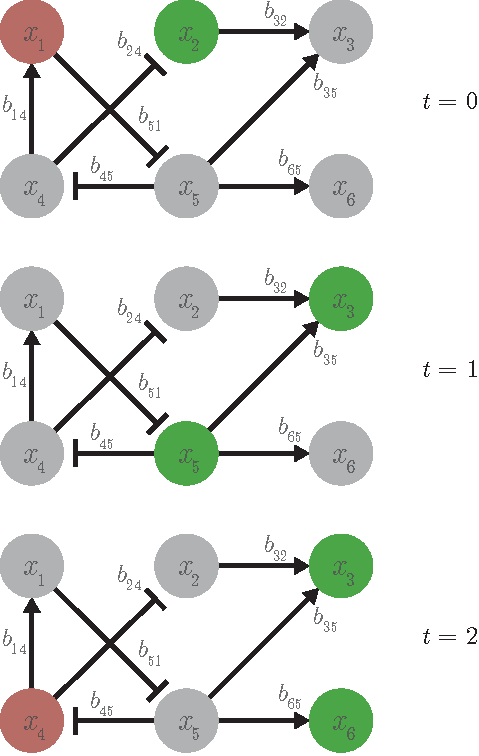
\includegraphics[width=.8\textwidth]{theory/fig/eberhardt.pdf}
    \caption{\textbf{Graph with constant edges.} \\ \textcolor{gray}{Gray} = 0, \textcolor{red!60!black}{red} < 0, \textcolor{green!45!black}{green} > 0.}
    \label{fig:eberhardt}
\end{figure}
\end{column}
\end{columns}
\end{frame}
\begin{frame}{Causality and cyclic graphs - Intervention}
\begin{columns}
\begin{column}{0.65\textwidth}
% We see that the convergence values are defined without referencing the node values at $t=0$ and the expression otherwise exactly matches~\autoref{eq:eber_linear.b}, except that taking a step forward or backward in time does not change the node values anymore.

% The diagonal of $B$ describes edges from nodes onto themselves, self-loops. These are unidentifiable from equilibrium data, since it is impossible to tell the difference between an node with a strong activator and a node with a weaker activator but a strong self-loop only based on steady-state gene expression levels. For this reason the diagonal of $B$ is always set to zeros. 

% The model is then expanded to include a concept of intervention of variables which in the context of biological network experiments is the equivalent of a knockout experiment of one or more genes. The intervention is the replacement of a node with a new value that follows standard Gaussian noise independent of the other variables in the network~(\autoref{eq:eber_intervention}).
Intervention
\begin{subequations}
\label{eq:eber_intervention}
\begin{align}
\boldsymbol{x}_k(t) &=
    U_k B \boldsymbol{x}_k(t-1) + U_k \boldsymbol{e} + \boldsymbol{c}_k
\\
\lim_{t \rightarrow \infty} \boldsymbol{x}_k(t) = \boldsymbol{x}_k &=
    (I - U_k B)^{-1} (U_k \boldsymbol{e} + \boldsymbol{c}_k)
\\
(I - U_k B) \boldsymbol{x}_k &=
    U_k \boldsymbol{e} + \boldsymbol{c}_k
\\
\label{eq:eber_intervention.d}
\boldsymbol{x}_k &=
    U_k B \boldsymbol{x}_k + U_k \boldsymbol{e} + \boldsymbol{c}_k
\end{align}
\end{subequations}
\end{column}
\begin{column}{0.35\textwidth}
\begin{figure}
    \centering
    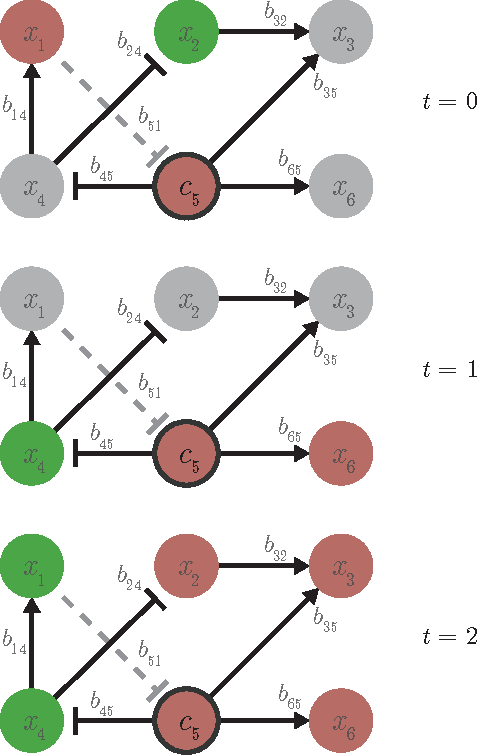
\includegraphics[width=.8\textwidth]{theory/fig/eberhardt_intervention.pdf}
    \caption{\textbf{Intervention on $x_5$.} \\ \textcolor{gray}{Gray} = 0, \textcolor{red!60!black}{red} < 0, \textcolor{green!45!black}{green} > 0.}
    \label{fig:intervention}
\end{figure}
\end{column}
\end{columns}
\end{frame}

\begin{frame}{Causality and cyclic graphs - $E[\boldsymbol{x}_k]$, covariance, and variable separation}
% The noise is given in $\boldsymbol{c}_k$ for the $k$-th experimental setup, where every value is zero except at the indexes of intervened nodes in experimental setup $k$. We refer to $k$ as an experimental setup rather than simply as an experiment to make it clear that the $k$-th experimental setup can be repeated multiple times, creating multiple observations of $\boldsymbol{x}_k$. The effect of other nodes onto the intervened variable is completely removed. 
% This makes sense in terms of a knockout where a removed gene will no longer be regulated by TFs. This is modelled using $U_k$ which is a diagonal matrix of ones, except at the indexes of intervened variables in experiment~$k$, where it has a value of zero. The result is the complete removal of the corresponding rows of $B$ and elements of $\boldsymbol{e}$. 
% A covariance matrix can be estimated if there are multiple observations for each experiment setup~$k$~(\autoref{eq:eber_cov}).
Expectation and covariance
\begin{subequations}
\label{eq:eber_cov}
\begin{align}
E[\boldsymbol{x}_k] &= (I-U_kB) ^{-1} \mu_{\boldsymbol{c}_k}
\\
\Sigma_{\boldsymbol{x}_k}
&=
\E \left[(\boldsymbol{x}_k - \E[\boldsymbol{x}_k] )(\boldsymbol{x}_k - \E[\boldsymbol{x}_k])^\trans \right]
\\
&= (I-U_kB)^{-1} E\left[ (U_k\boldsymbol{e}_k + \boldsymbol{c}_k - \mu_{\boldsymbol{c}_k})(U_k\boldsymbol{e}_k + \boldsymbol{c}_k - \mu_{\boldsymbol{c}_k})^\trans \right] (I-U_kB)^{-\trans}
\\
&= (I-U_kB)^{-1} (\Sigma_{\boldsymbol{c}_k} + U_k\Sigma_{\boldsymbol{e}} U_k) (I-U_kB)^{-\trans}
\end{align}
\end{subequations}
% Where $\mu_{\boldsymbol{c}_k}$ is the expected value of $\boldsymbol{c}_k$, and $\Sigma_{\boldsymbol{x}_k}$ is the covariance matrix of $\boldsymbol{x}_k$. The interesting parts of the covariance matrix are the entries describing covariance between the intervened variables and the passively observed variables. Since it is assumed that no variable has an effect onto intervened variables it can be possible to describe the observed covariance as more than just an undirected covariance edge between the two nodes but instead as a directed edge of causality from the intervened to the non-intervened.
% We denote the elements of vectors and matrices with subscript $\mathcal{J}_k$, $\mathcal{U}_k$, and $\mathcal{V}$ to refer to indexes for nodes intervened on in experimental setup $k$, passively observed in experimental setup $k$ and indexes of all nodes, respectively. We split our expression for $\boldsymbol{x}_k$ from \autoref{eq:eber_intervention.d} into expressions for intervened and non-intervened variables~(\autoref{eq:JU}).
Separating intervened ($\boldsymbol{x}_{\mathcal{J}_k}$) and passively observed ($\boldsymbol{x}_{\mathcal{U}_k}$) variables
\begin{subequations}
\label{eq:JU}
\begin{align}
\boldsymbol{x}_{\mathcal{J}_k} &= \boldsymbol{c}_{\mathcal{J}_k}
\\
\boldsymbol{x}_{\mathcal{U}_k} &= B_{\mathcal{U}_k\mathcal{V}} \boldsymbol{x}_k + \boldsymbol{e}_{\mathcal{U}_k}
\\
&= B_{\mathcal{U}_k\mathcal{U}_k} \boldsymbol{x}_{\mathcal{U}_k} + B_{\mathcal{U}_k\mathcal{J}_k} \boldsymbol{x}_{\mathcal{J}_k} + \boldsymbol{e}_{\mathcal{U}_k}
\\
(I - B_{\mathcal{U}_k\mathcal{U}_k}) \boldsymbol{x}_{\mathcal{U}_k} &=
B_{\mathcal{U}_k\mathcal{J}_k}\boldsymbol{x}_{\mathcal{J}_k} + \boldsymbol{e}_{\mathcal{U}_k}
\\
\boldsymbol{x}_{\mathcal{U}_k} &=
(I - B_{\mathcal{U}_k\mathcal{U}_k})^{-1}(B_{\mathcal{U}_k\mathcal{J}_k}\boldsymbol{x}_{\mathcal{J}_k} + \boldsymbol{e}_{\mathcal{U}_k})
\end{align}
\end{subequations}
\end{frame}

\begin{frame}{Causality and cyclic graphs - Covariance between $\boldsymbol{x}_{\mathcal{J}_k}$ and $\boldsymbol{x}_{\mathcal{U}_k}$}
% The covariance between $\boldsymbol{x}_{\mathcal{J}_k}$ and $\boldsymbol{x}_{\mathcal{U}_k}$ can then be described~(\autoref{eq:causal_cov}).
Covariance between intervened ($\boldsymbol{x}_{\mathcal{J}_k}$) and passively observed ($\boldsymbol{x}_{\mathcal{U}_k}$) variables
\begin{subequations}
\label{eq:causal_cov}
\begin{align}
(\Sigma_{\boldsymbol{x}_k})_{\mathcal{J}_k\mathcal{U}_k} &=
\E \left[ (\boldsymbol{x}_{\mathcal{J}_k} - \E[\boldsymbol{x}_{\mathcal{J}_k}])
(\boldsymbol{x}_{\mathcal{U}_k} - \E[\boldsymbol{x}_{\mathcal{U}_k}])^\trans \right]
\\
&= \E \left[
(\boldsymbol{x}_{\mathcal{J}_k} - \E[\boldsymbol{x}_{\mathcal{J}_k}])
(B_{\mathcal{U}_k\mathcal{J}_k} (\boldsymbol{x}_{\mathcal{J}_k} - \E[\boldsymbol{x}_{\mathcal{J}_k}]))^\trans
\right]
(I - B_{\mathcal{U}_k\mathcal{U}_k})^{-\trans}
\\
&= (\Sigma_{\boldsymbol{c}_k})_{\mathcal{J}_k\mathcal{J}_k} B^\trans_{\mathcal{U}_k\mathcal{J}_k} (I - B_{\mathcal{U}_k\mathcal{U}_k})^{-\trans}
\end{align}
\end{subequations}
% Eberhardt~et~al. deals with what they call canonical experiments to simplify notation where each element in $\boldsymbol{c}_k$ is uncorrelated with zero mean and unit variance. From this and the symmetry of covariance matrices we get expression for covariance between intervened and passively observed that only depend on entries of $B$~(\autoref{eq:eberhardt_cov}). Matrix $T_{\boldsymbol{x}_k}$ is also introduced here.
Using i.i.d. interventions $\boldsymbol{c}_k$
\begin{subequations}
\label{eq:eberhardt_cov}
\begin{align}
(\Sigma_{\boldsymbol{c}_k})_{\mathcal{J}_k\mathcal{J}_k} &= I
\\
(\Sigma_{\boldsymbol{x}_k})_{\mathcal{J}_k\mathcal{U}_k} &= B^\trans_{\mathcal{U}_k\mathcal{J}_k} (I - B_{\mathcal{U}_k\mathcal{U}_k})^{-\trans}
= T_{\boldsymbol{x}_k}^\trans
\\
(\Sigma_{\boldsymbol{x}_k})_{\mathcal{U}_k\mathcal{J}_k} &=
T_{\boldsymbol{x}_k} =
(I - B_{\mathcal{U}_k\mathcal{U}_k})^{-1} 
B_{\mathcal{U}_k\mathcal{J}_k} 
\end{align}
\end{subequations}
\end{frame}

\begin{frame}{Causality and cyclic graphs - Experimental effect}
% A concept of the overall effect from node $x_i$ to $x_u$, referred to as "experimental effect", is introduced~(\autoref{eq:experimental_effect}). It should be read as the total experimental effect from $x_i$ on $x_u$ given the conditions where $\mathcal{J}_k$ refers to the indexes of intervened variables in experimental setup $k$.
Total effect from $x_i$ to $x_u$ is sum of all directed paths
\begin{subequations}
\label{eq:experimental_effect}
\begin{align}
t(x_i \rightsquigarrow x_u || \mathcal{J}_k) &= \sum_{p \in \mathcal{P}(x_i \rightsquigarrow x_u || \mathcal{J}_k)} \prod_{(x_l \rightarrow x_m) \in p} b_{ml}
\\
\label{eq:t_to_b}
&= b_{ui} + \sum_{x_j \in \mathcal{U}_k \setminus \{x_u\}} t(x_i \rightsquigarrow x_j || \mathcal{J}_k) b_{uj}
\end{align}
\end{subequations}

% It is defined as summing the effects from each path from $x_i$ to $x_u$, where the effect along a given path is simply the product over all edge values $b_{ml}$ along that path. Since the graph has cycles there can be an infinite number of paths connecting $x_i$ and $x_u$. 

% In appendix C of 
Eberhardt~et~al.~\cite{EberhardtLLCdetail} proves
\begin{equation}
    t(x_i \rightsquigarrow x_u || \mathcal{J}_k) = (T_{\boldsymbol{x}_k})_{\{x_u\}\{x_i\}}
\end{equation}

%, which means that the experimental effect is equal to the element $u,i$ of the covariance matrix in the case where $x_i$ is intervened upon and $x_u$ is not. The empirical covariance matrix of observed variables can be used as an approximation of the true covariance matrix and thereby used for finding $t(x_i \rightsquigarrow x_u || \mathcal{J}_k)$ for different indexes of $i$ and $u$. As formulated in \autoref{eq:t_to_b} the values of $t(x_i \rightsquigarrow x_u || \mathcal{J}_k)$ are related to the values of $B$ where multiple observations can form a linear system of equations to solve for $B$.
% The resulting LLC algorithm does exactly this.
LLC (Linear, Latent, Cyclic) algorithm overview
\begin{equation}
\Sigma_{\boldsymbol{x}_k}
\rightarrow
T_{\boldsymbol{x}_k}
\rightarrow
t(x_i \rightsquigarrow x_u || \mathcal{J}_k)
\rightarrow
B
\end{equation}
% An issue arises when the covariance matrix cannot be estimated as is the case if there is only a single observation of $\boldsymbol{x}_k$ for each experimental setup $k$. $t(x_i \rightsquigarrow x_u || \mathcal{J}_k)$ is considered a regression coefficient when regressing $x_u$ over the only manipulated variable $x_i$, which means it is calculated as a linear regression coefficient where each observation is treated as the expected value~(\autoref{eq:t_regress}).
If covariance is unknown
\begin{equation}
\label{eq:t_regress}
t(x_i \rightsquigarrow x_u || \{x_i\}) \cdot x_i = x_u
\implies
t(x_i \rightsquigarrow x_u || \{x_i\}) = \frac{x_u}{x_i}
\end{equation}

% LLC is available as \texttt{R}-code, which was used for the $B$-method introduced in~\autoref{sec:equilibrium_inference}.


\end{frame}


\begin{frame}<0>{Inference helped by evolution}
\label{sec:evolution}
% The one you were supposed to have used is "Improving gene network inference by comparing expression time-series across species, developmental stages or tissues" by Guillaume Bourque and David Sankoff from Canada.
Interspecies data
\begin{itemize}
    \item protein interactions
    \item sequence data~\cite{KEGG}
% Interspecies data and other data sources can be included in the effort of protein interaction and gene regulation inference. Protein interaction data from other species can be used on the expectation that if a protein interaction exists in one species, the orthologous proteins are likely to interact in a different species. Genetic and amino acid sequence data can also be exploited by studying the genetic or amino acid similarities to that of another species, and basing expectations of similarity in protein interaction properties on similarity observed in the orthologous proteins' sequences. Gene and amino acid sequences can be obtained from the KEGG GENES database~\cite{KEGG}.
\end{itemize}
Metabolic networks by Kashima~et~al.~\cite{Kashima2009}
\begin{itemize}
    \item Incomplete protein interactions ($\text{A}^{(k)}$)
    \item interspecies protein similarity ($\text{W}^{(k,l)}, k \ne l$)
    \item intraspecies gene expression similarity ($\text{W}^{(k,l)}, k = l$)
\end{itemize}
% Inference of metabolic networks has been studied, where the metabolic networks were treated as a graph for each species~\cite{Kashima2009}. Nodes are enzymes and edges are undirected, representing enzyme reactions in a metabolic pathway.
% Incomplete adjacency matrices $\text{A}^{(k)}$ were obtained for each species $k$, where values indicate presence, absence, or unknown status of enzyme interactions. Sequence similarities for all pairs of proteins were used for calculation of protein similarity scores as symmetrical positive matrices $\text{W}^{(k,l)}$ comparing species $k$ and $l$, where $k\ne l$. Gene expression profiles from DNA microarray hybridization measurements were used for intraspecies similarity matrices $\text{W}^{(k,l)}$, where $k=l$. 
% The idea is to find pairs of orthologous enzymes in different species where their presence or absence of interaction is known for one species but not for the other, and then score the interaction accordingly for the species with incomplete edge information. This is done with $\Tilde{\text{W}}^{(k,l)} = \text{W}^{(k,l)} \otimes \text{W}^{(k,l)}$, where $\otimes$ is the Kronecker product. $\Tilde{\text{W}}^{(k,l)}$ holds the product of each combination of elements of $\text{W}^{(k,l)}$, thereby scoring each enzyme interactions based on how likely it is that the two enzymes involved are orthologous.
% Edge scoring matrices were then inferred by minimizing a loss function that depends on each~$\Tilde{\text{W}}^{(k,l)}$, and~$\text{A}^{(k)}$. Naturally, edges are only inferred for incomplete entries in the adjacency matrices.
% Sequence similarity data could similarly be applied in combination with knockout data for more comprehensive graph inference for signal transduction networks.
\end{frame}


